\section{Residual Analysis}

We now consider the residuals for some of the models we previously fit. To create the residual plot for l.tankregression we used the `broom' package \citep{broom}.


\begin{figure}[H]
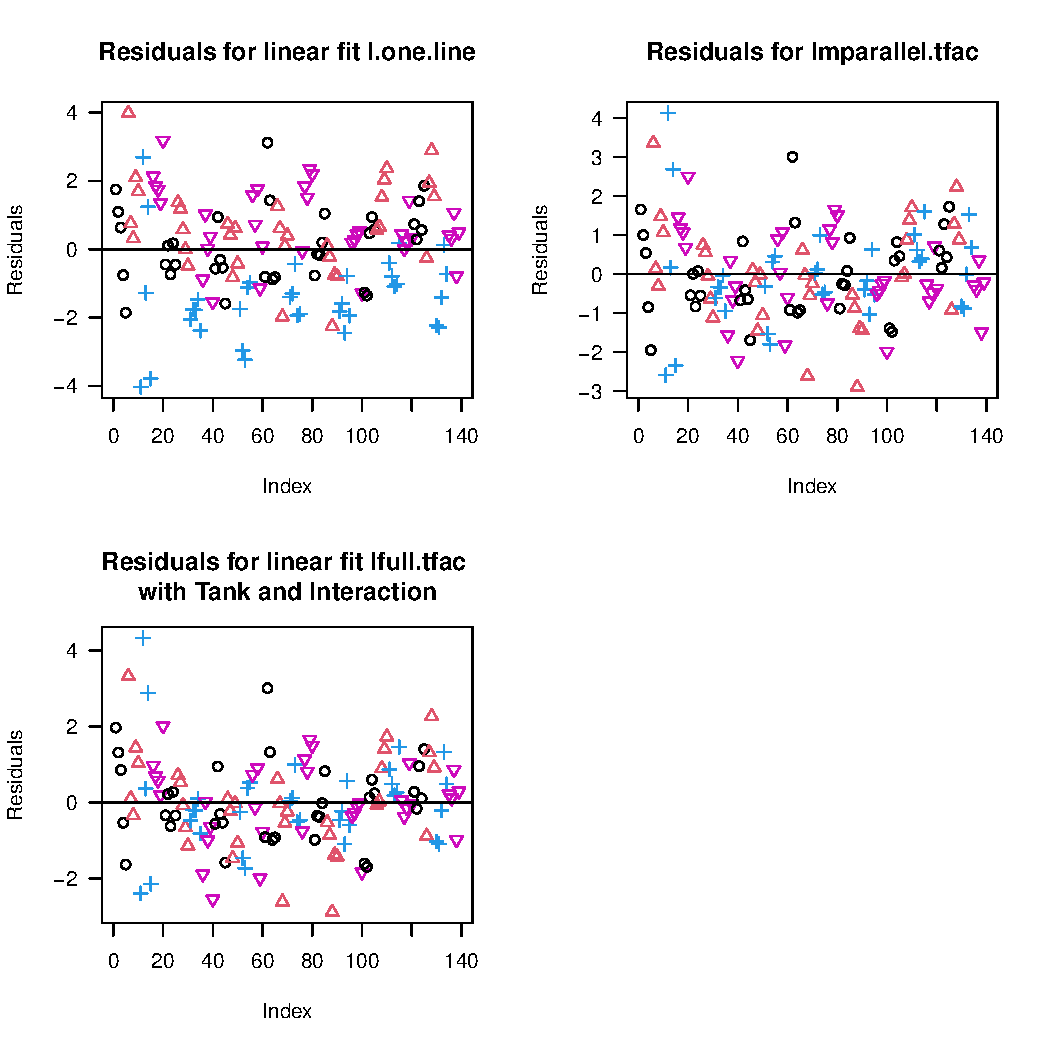
\includegraphics[scale=0.9]{Chapter3Images/residuals2.pdf}
\caption{ \hspace{1mm} Residual plots for three models, l.one.line, lmparallel.tfac and lfull.tfac are the standard linear models for median TCT. Tanks 19, 20, 21 and 24 are represented as black circles, red triangles, blue crosses and pink inverted triangles respectively. }
\label{lab:resid2}
\end{figure}



\begin{figure}[H]
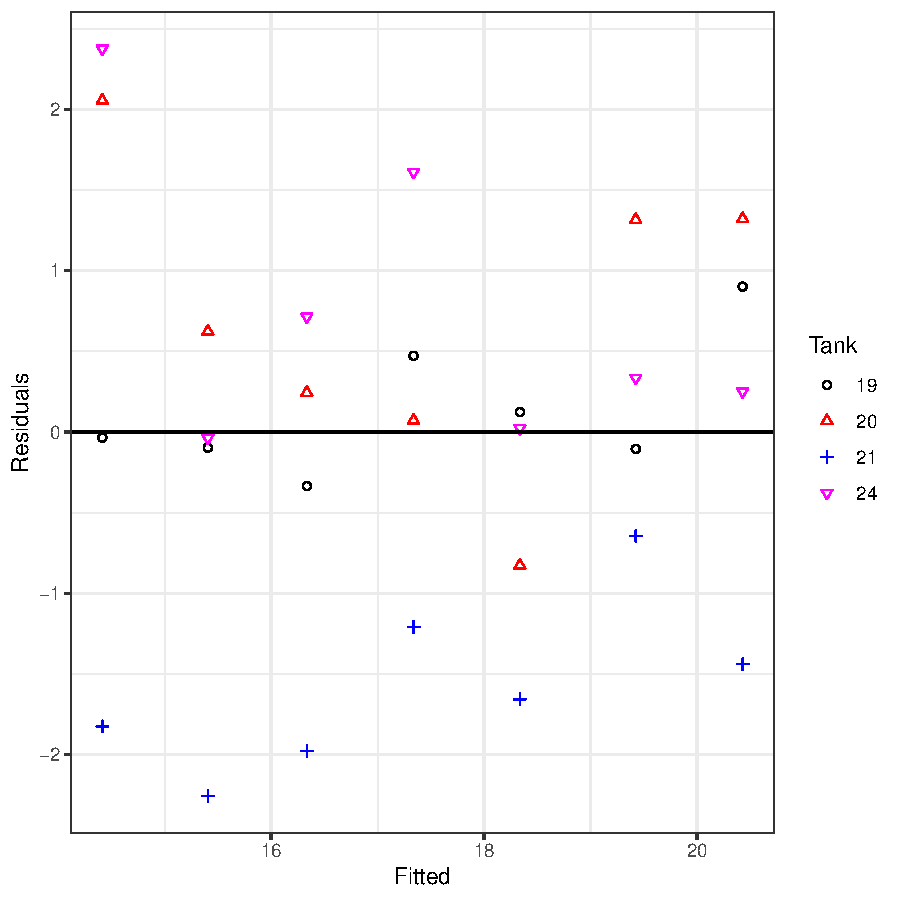
\includegraphics{Chapter3Images/ltankregressionresid.pdf}
\caption{ This image shows the basic residual plot for our final chosen model for mean TCT, l.tankregression.}
\label{lab:resid22}
\end{figure}

Figure~\ref{lab:resid2} shows the residuals from three of the models we fit. The residuals appear to be randomly distributed about the x-axis which is a good indication that our model is making valid assumptions. Figure~\ref{lab:resid22} is a plot of the residuals for l.tankregression. The residuals again appear to be randomly distributed about the x-axis. Although Tank 21 has consistently negative residuals. The legend indicates which tank each point belonged to.


